\section{Evaluation}
\label{sec:evaluation}

Testbed settings..

\subsection{Microbenchmarks}

Figure~\ref{fig:eval-conn-setup-tput} shows throughput of connection creation. Key points: a) FastSocket not fast enough, b) higher throughput, c) scalable with number of cores.

Figure~\ref{fig:eval-msgsize-intra} shows throughput and latency with different message sizes for intra-server communication. Key points: a) shared memory is faster than NIC hairpin, b) user space is faster than kernel, c) zero copy for large messages.

Figure~\ref{fig:eval-msgsize-inter} shows throughput and latency with different message sizes for inter-server communication. Key points: a) RDMA is faster than DPDK + user-space stack, b) zero copy for large messages.

Figure~\ref{fig:eval-connnum-tput} shows throughput with different number of concurrent connections (log scale on x axis). Key points: a) SocksDirect is scalable with number of connections, b) other systems with one queue per socket has performance degradation under high concurrency.

Figure~\ref{fig:eval-cornum-ipc} shows throughput with different number of cores for intra-server communication. Key points: a) SocksDirect is scalable with number of cores, b) NIC hairpin is not scalable with number of cores.

Table~\ref{tab:eval-context-switch} shows throughput and latency with a dispatcher process on core $A$, multiple worker processes on core $B$ and a reducer process on core $C$. Key points: a) When all workers are active, throughput is comparable with single worker. b) When only a fraction of workers are active, the idle workers do not impact performance. c) Latency increases with number of active workers, but still much lower than Linux.


\begin{figure}[htpb]
	\centering
	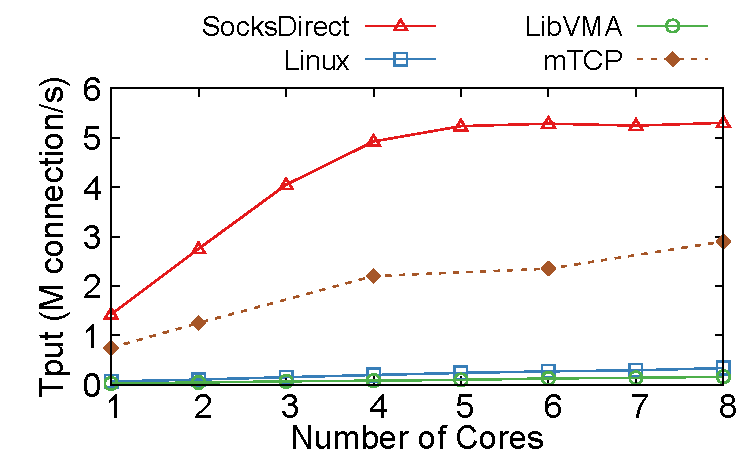
\includegraphics[width=\columnwidth]{eval/microbenchmark/conn-setup-tput.pdf}
	\caption{Throughput of the connection creation}
	\label{fig:eval-conn-setup-tput}
\end{figure}


\begin{figure}[htpb]
	\centering
	\subfloat[Intra-server throughput]{                    
		%\begin{minipage}{0.4\textwidth}
		\centering
		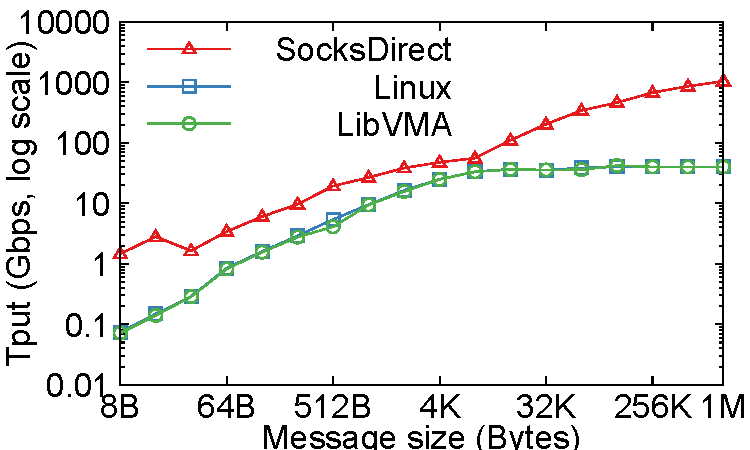
\includegraphics[width=\columnwidth]{eval/microbenchmark/msgsize-ipc-tput.pdf}
		\label{fig:eval-msgsize-ipc-tput}
		%\end{minipage}
	}
	
	\subfloat[Intra-server latency]{
		%\begin{minipage}{0.4\textwidth}
		\centering 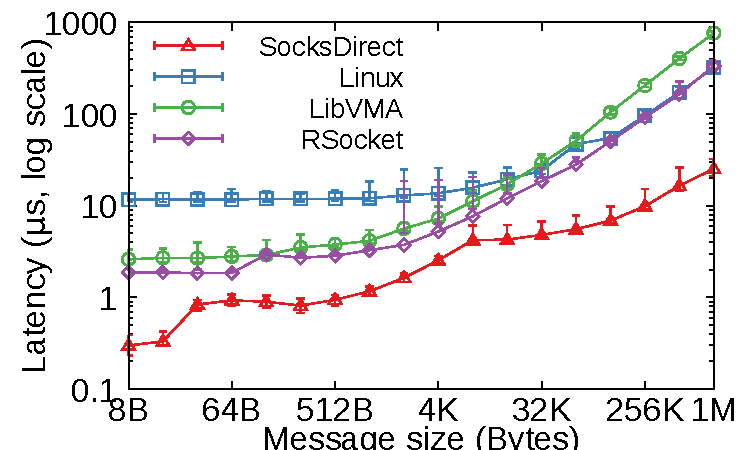
\includegraphics[width=\columnwidth]{eval/microbenchmark/msgsize-ipc-lat.pdf}
		\label{fig:eval-msgsize-ipc-lat}
		%\end{minipage}
	}
	\caption{Intra-server performance with different message sizes}
	\label{fig:eval-msgsize-intra}
\end{figure}

\begin{figure}[htpb]
	\centering
	\subfloat[Inter-server throughput]{
		%\begin{minipage}{0.4\textwidth}
		\centering 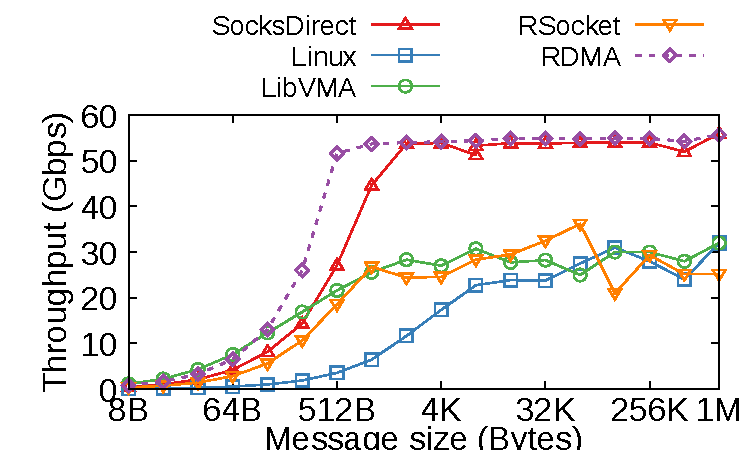
\includegraphics[width=\columnwidth]{eval/microbenchmark/msgsize-network-tput.pdf}
		\label{fig:eval-msgsize-network-tput}
		%\end{minipage}
	}
	
	\subfloat[Inter-server latency]{
		%\begin{minipage}{0.4\textwidth}
		\centering 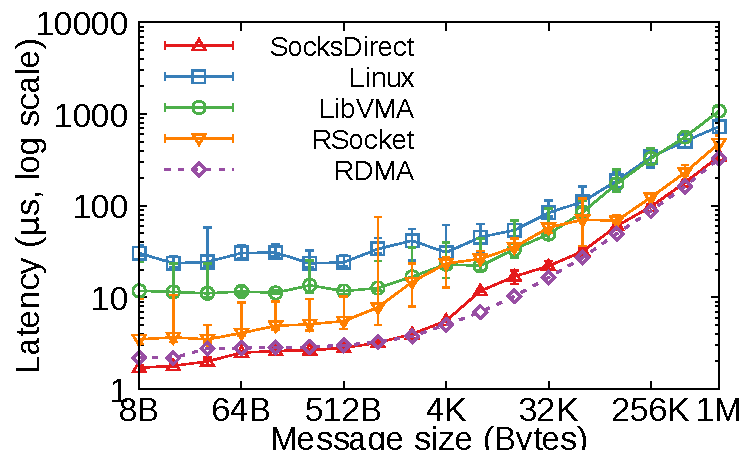
\includegraphics[width=\columnwidth]{eval/microbenchmark/msgsize-network-lat.pdf}
		\label{fig:eval-msgsize-network-lat}
		%\end{minipage}
	}
	\caption{Inter-server performance with different message sizes}
	\label{fig:eval-msgsize-inter}
\end{figure}

\begin{figure}[htpb]
\centering                                                         
\subfloat[Intra-server]{                    
	%\begin{minipage}{0.4\textwidth}
	    \centering
	    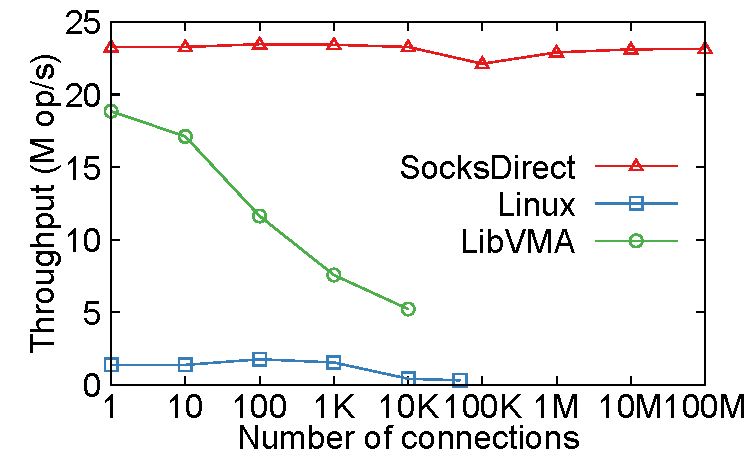
\includegraphics[width=\columnwidth]{eval/microbenchmark/connnum-ipc-tput.pdf}
	    \label{fig:eval-connnum-ipc-tput}
	%\end{minipage}
	}

\subfloat[Inter-server]{
	%\begin{minipage}{0.4\textwidth}
		\centering 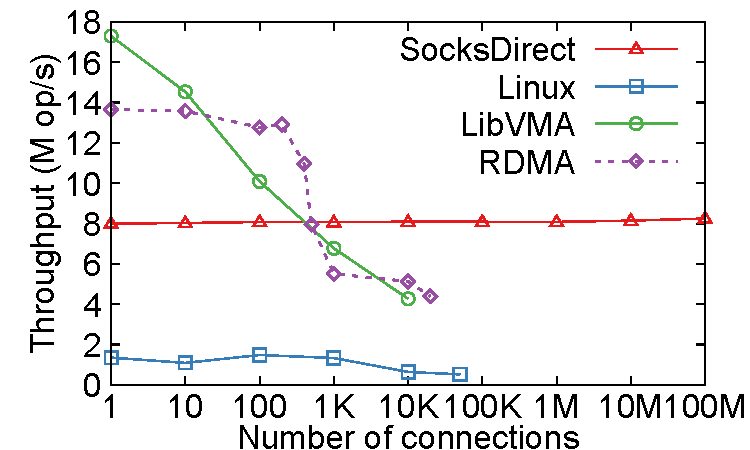
\includegraphics[width=\columnwidth]{eval/microbenchmark/connnum-network-tput.pdf}
		\label{fig:eval-connnum-network-tput}
	%\end{minipage}
	}
	\caption{Throughput with different number of connections}
	\label{fig:eval-connnum-tput}
\end{figure}

\begin{figure}[htpb]
	\centering
	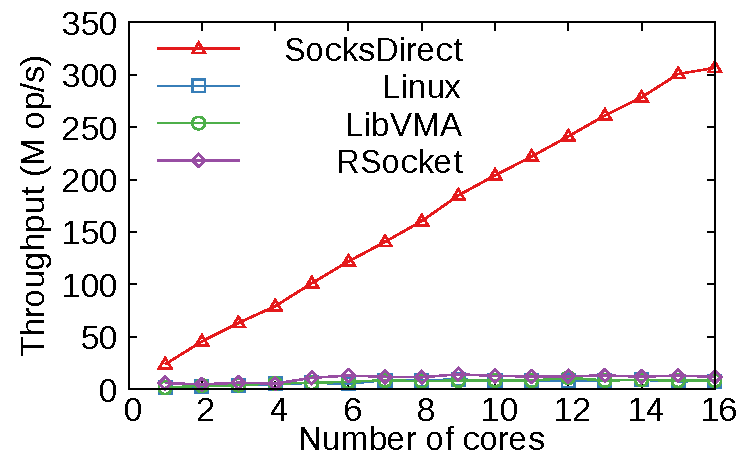
\includegraphics[width=\columnwidth]{eval/microbenchmark/corenum-IPC-tput.pdf}
	\caption{Throughput with different number of cores for intra-server communication}
	\label{fig:eval-cornum-ipc}
\end{figure}

\begin{table}[t]
	\centering
		\begin{tabular}{l|c|c|c|c|c|c|}
			\hline
				& \multicolumn{3}{c|}{Throughput} & \multicolumn{3}{c|}{Latency} \\
			\hline
			Num of Workers	& \multicolumn{1}{c|}{1} & \multicolumn{2}{c|}{8} & \multicolumn{1}{c|}{1} & \multicolumn{2}{c|}{8} \\
			\hline
			Num of Active Workers	& 1 & 1 & 8 & 1 & 1 & 8 \\
			\hline
			\hline
			SocksDirect 	& 1 & 1 & 8 & 1 & 1 & 8 \\
			\hline
			Linux 	& 1 & 1 & 8 & 1 & 1 & 8 \\
			\hline
		\end{tabular}
	\caption{Performance evaluation of multiple processes sharing a core.}
	\label{tab:eval-context-switch}
\end{table}



\subsection{Network Function}

Network functions~\cite{li2016clicknp}, ClickOS~\cite{martins2014clickos}

Scenarios: Firewall (no packet change), NAT (change a packet field), Tunnel endpoint (add/remove packet header, change length)

Metrics: Latency, throughput

\begin{figure}[htpb]
	\centering
	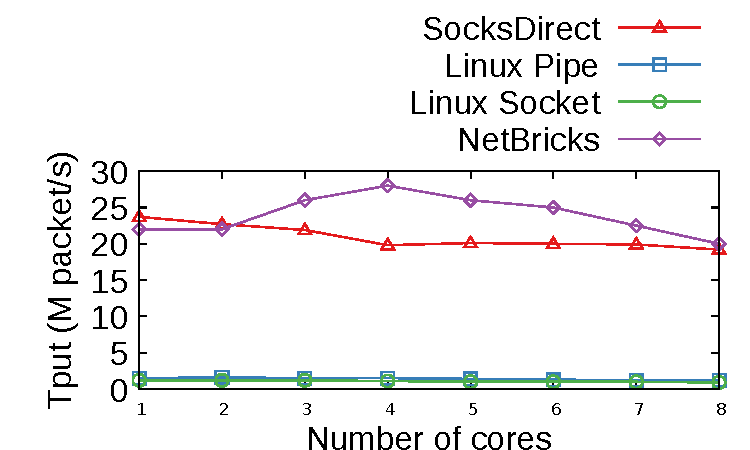
\includegraphics[width=\columnwidth]{eval/microbenchmark/nfv-tun-tput.pdf}
	\caption{Throughput of NFV tunnel}
	\label{fig:eval-tun-tput}
\end{figure}



\subsection{Web Application}

Nginx~\cite{nginx}, Nodejs~\cite{nodejs} and memcached~\cite{memcached}

\begin{itemize}
	\item Figure~\ref{fig:eval-nginx-short}: Many short-lived connections. Nginx $\rightarrow$ Nodejs, Nodejs access memcached once.
	\item Figure~\ref{fig:eval-nginx-multiround}: Each connection, backend interact extensively. (Nodejs access memcached multiple round trips.)
	\item Figure~\ref{fig:eval-nginx-long}: Long connection to download a large in-memory file. (test zero copy)
\end{itemize}

\begin{figure}[htpb]
	\centering                                                         
	\subfloat[Throughput of Simple Short-lived connections]{                    
		%\begin{minipage}{0.4\textwidth}
			\centering
			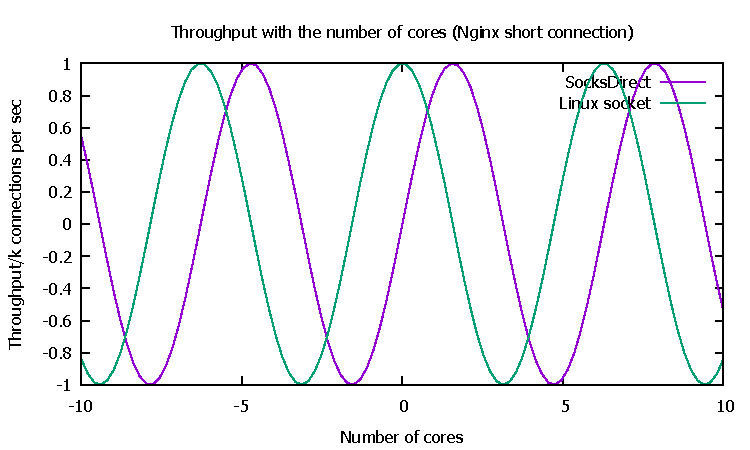
\includegraphics[width=\columnwidth]{eval/microbenchmark/nginx-short-tput.pdf}
			\label{fig:eval-nginx-short}
		%\end{minipage}
		}
	
	\subfloat[Latency of complicated requests]{
		%\begin{minipage}{0.4\textwidth}
			\centering 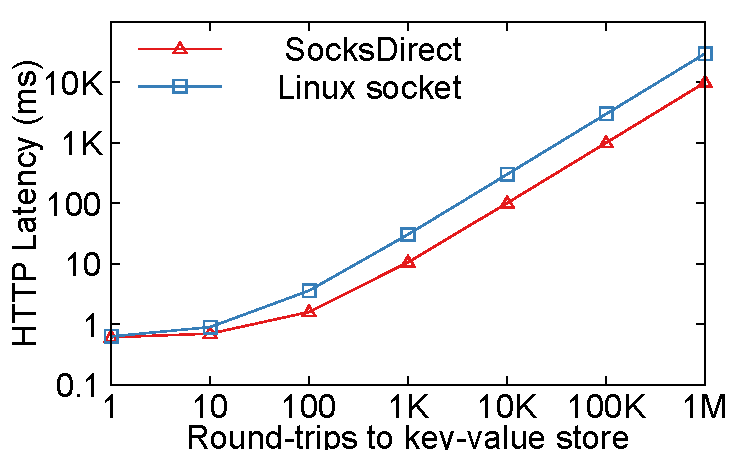
\includegraphics[width=\columnwidth]{eval/microbenchmark/nginx-multiround-tput.pdf}
			\label{fig:eval-nginx-multiround}
		%\end{minipage}
		}

		\subfloat[Transmission throughput of a long-lived connection]{
		%\begin{minipage}{0.4\textwidth}
			\centering 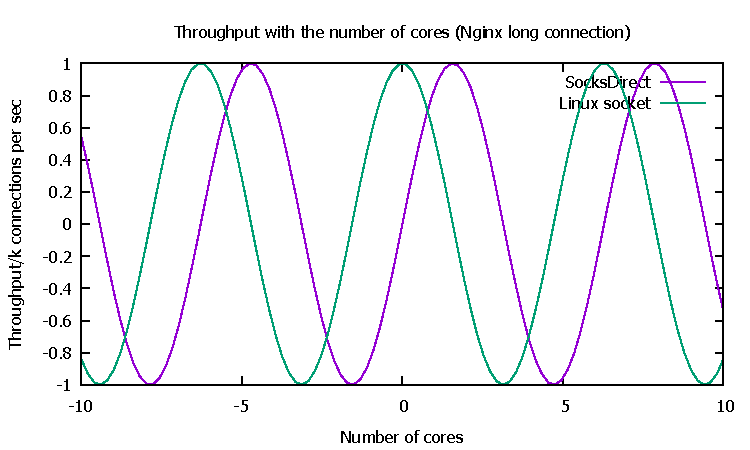
\includegraphics[width=\columnwidth]{eval/microbenchmark/nginx-long-tput.pdf}
			\label{fig:eval-nginx-long}
		%\end{minipage}
		}
		
		\caption{Performance of a web service composed of Nginx, Node.js and memcached.}
		\label{fig:eval-nginx-tput}                                           
\end{figure}


%\subsection{Real-time Stream Processing}

%Apache Flink~\cite{carbone2015apache} (need to turn off durability on disk)

%Scenario: Word Count (distributed system with one source, two mappers and one reducer)

%Metrics: Latency, throughput

%\subsection{Machine Learning}

%Tensorflow~\cite{abadi2016tensorflow}

%Scenario: (Distributed Tensorflow) Parameter server and worker on a same server.

%Metrics: Time per iteration